\documentclass{article}

\usepackage[dblblindworkshop]{neurips_2026}
\workshoptitle{Sim2Science}

\usepackage[utf8]{inputenc}
\usepackage[T1]{fontenc}
\usepackage{hyperref}
\usepackage{url}
\usepackage{booktabs}
\usepackage{amsfonts}
\usepackage{amsmath}
\usepackage{nicefrac}
\usepackage{microtype}
\usepackage{graphicx}
\usepackage{xcolor}

\newcommand{\Fone}{$F_1$}
\newcommand{\Ftwo}{$F_2$}
\newcommand{\Treal}{$T$}

\title{How Wrong Can Your Simulator Be? Auditing, Tolerating, and Updating a Measured Forward Model on a Real Instrument}

\author{%
  Anonymous Author(s)
}

\begin{document}

\maketitle

\begin{abstract}
A learned restoration model for degraded macro X-ray fluorescence (MA-XRF) scans of a painting is trained on a forward simulator whose every ingredient (geometry, per-line gains, noise law) is measured on the instrument; we treat the simulator's imperfection as the object of study. An ensemble trained across simulators drawn within the measured calibration uncertainty separates simulator uncertainty from initialisation variance (2.8$\times$ wider than a fixed-simulator control on the real scan, 86\,\% of its variance attributable to the simulator), yields a near-calibrated band on the real scan (coverage 0.61/0.87/0.95 at 1/2/3$\sigma$), and its mean is the first learned restoration in our study that does not lose correlation to the physics inverse on the real scan. A ladder of 18 deliberately broken training simulators shows the learned refinement tolerates large noise and gain errors but fails on geometry: 0.5\,px of registration error already hurts, and 1\,px makes the network worse than the physics it refines. A blind diagnostic battery, thresholded on the calibration uncertainty itself, identifies every defect that causes material damage, and on the real scan rediscovers, unsupervised, the resampling-blur mismatch that had originally broken our training pipeline. Used as ABC summaries, the same statistics turn one real scan into a posterior over the simulator: the blur defect is rejected (prior probability 0.5, posterior 0.000) and a posterior-trained ensemble is the most accurate restoration in the study, with a 27\,\% narrower band than the prior ensemble. Finally, a 180-case degradation grid with four classical inpainting controls shows where learning pays: everywhere on measured pixels, nowhere inside missing regions, where a biharmonic fill wins in 16 of 16 cells. All results are anchored on real measurements from one instrument and one painting; all negative results are reported.
\end{abstract}

\section{Introduction}
\label{sec:intro}

Machine learning for experimental science usually trains on simulations because ground truth is scarce, and the simulator is never exactly the instrument; the common response is to validate it once and trust it. This paper takes the opposite view on a small but fully measured problem: we ask \emph{how} imperfect a validated simulator still is, what that imperfection costs a network trained on it, whether it can be detected and attributed blind, how to represent it honestly in predictive uncertainty, and whether a single real measurement can reduce it.

Our testbed is the restoration of geometrically degraded MA-XRF element maps of an oil painting \citep{alfeld2013}: a scan acquired at a tilt must be registered, gain-corrected and denoised back into the frontal frame. The forward model is not designed but measured (Section~\ref{sec:setup}), which gives us something rare: a per-component calibration uncertainty for every knob of the simulator. Our contributions:

\begin{itemize}
  \item \textbf{Uncertainty that knows the simulator is imperfect.} Deep ensembles \citep{lakshminarayanan2017} trained across simulator draws within the measured calibration uncertainty, against a fixed-simulator control that isolates initialisation variance (Section~\ref{sec:wp1}): domain randomization \citep{tobin2017} with measured ranges, evaluated as uncertainty quantification.
  \item \textbf{A defect-tolerance ladder and a blind audit.} One network per deliberately broken simulator quantifies which defects hurt; a battery of summary statistics, thresholded on the calibration uncertainty, identifies which component is broken without ground truth (Section~\ref{sec:wp2}). Every defect that causes material damage is visible to the audit.
  \item \textbf{Closing the loop.} The audit statistics are ABC summaries \citep{beaumont2002,cranmer2020}: one real scan yields a posterior over the simulator's knobs, a posterior-trained ensemble, and a posterior predictive check that names precisely what the simulator still lacks (Section~\ref{sec:wp4}).
  \item \textbf{A regime map against classical baselines.} A 180-case grid over tilt, missing data and dose, with four classical inpainting controls, locates the frontier where learning pays (Section~\ref{sec:wp3}); inside missing regions the answer is unflattering and we report it as such.
\end{itemize}

\section{Setup: a measured forward model, and how it burned us}
\label{sec:setup}

\paragraph{Instrument and data.} Two silicon drift detectors (70\,mm$^2$ mounted horizontally and 25\,mm$^2$ at 40$^\circ$ from horizontal, 12.5\,\textmu m Be windows) and a tube at 37\,kV / 40\,\textmu A scan an oil painting; per-pixel spectra are fitted into net-count maps of 8 element lines (Ca, Ti, Fe, Cu, and four Pb\,L lines), summed over the detectors. Scans: two frontal, \Fone{} and \Ftwo{} ($60\times120$ px, seven days apart, same geometry), and one real tilted, \Treal{} ($45\times80$, mounted at 7.7$^\circ$). \Fone{} is the only training source; \Ftwo{} and \Treal{} are reserved for evaluation and are never seen in training.

\paragraph{Forward model.} Every ingredient is measured, not modelled: the warp is the affine registration fitted between \Treal{} and \Fone{}; the per-line tilt gains are the measured level response at the reference mounting, extrapolated linearly in angle; the noise is Poisson-consistent with a per-line constant, $\mathrm{Var}(m) = k_{\mathrm{el}} m$ with $k_{\mathrm{el}}\!=\!4.2$--$9.0$ calibrated from the \Fone{}--\Ftwo{} difference. A fidelity gate holds on all 8 lines: $r(\mathrm{sim},\Treal{}) = 0.89$--$0.98$, within 0.02 of the \Fone{}--\Ftwo{} repeatability ceiling, and levels within 0.7\,\%. A residual U-Net \citep{ronneberger2015} (469k parameters, zero-initialised head, so the untrained network \emph{is} the physics inverse) refines the deterministic inversion; training pairs are simulated from \Fone{} at random angles, doses and dropout blocks (Appendix~\ref{app:training}).

\paragraph{The blur lesson.} Our first training simulator emulated the tilted acquisition by bilinearly warping the frontal map. It passed the fidelity gate, yet the network trained on it \emph{over-sharpened} the real scan (contrast ratio up to 1.05, correlation below the physics inverse on 8/8 lines). The cause: a real tilted scan is a direct measurement and carries no resampling blur, so the simulated restoration inputs carried two interpolation blurs where reality has one. Sampling the source with a cubic spline at the exact warp positions (v2) fixed the training distribution. The lesson behind everything below: \emph{validated as an emulator is not validated as a training-data generator}, and the failure was invisible on simulated tests.

\paragraph{Perturbable simulator.} We expose the simulator's components as knobs $\theta$: a noise-constant scale, a tilt-gain slope scale, per-line gain offsets, the assumed mounting angle, registration shift and rotation, the interpolation order (cubic vs the v1 bilinear), and, in Section~\ref{sec:wp4}, per-line noise scales. Each knob carries a measured 1$\sigma$ calibration uncertainty (noise log-sd 0.33 from the session transfer of $k$; gain slope 20\,\%, the mounting angle being an upper bound; registration 0.1\,px, 0.3$^\circ$ from the spread of per-element fits). Perturbations apply only to the training-data simulator; the test-time inverse stays nominal, as in practice.

\section{Uncertainty that knows the simulator is imperfect}
\label{sec:wp1}

\begin{figure}[t]
  \centering
  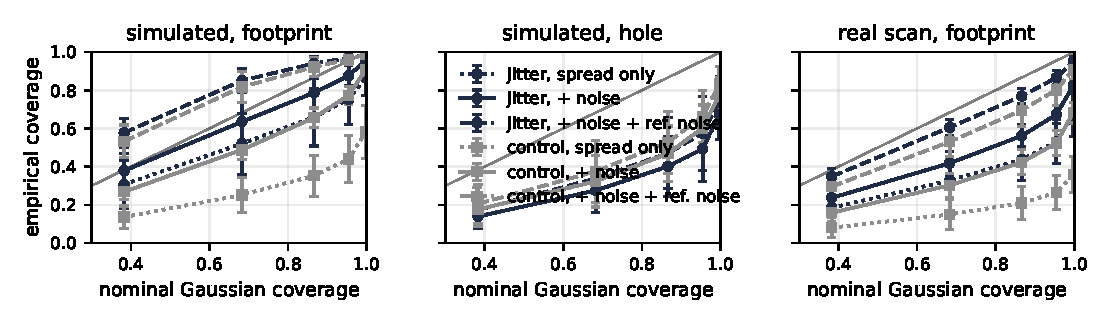
\includegraphics[width=0.75\linewidth]{wp1_calibration.pdf}
  \caption{Coverage of $|\mathrm{mean}-\mathrm{truth}|\le z\sigma$ vs the Gaussian target, jitter (navy) and control (grey); dotted: spread only, solid: plus propagated noise, dashed: plus reference-map noise (upper bound on simulated cases, the correct band on the real scan). Bars: sd over lines and cases. Left: 32 simulated cases (footprint); middle: inside a $14\times20$ hole; right: the real scan.}
  \label{fig:calibration}
\end{figure}

We train two ensembles of $N{=}12$ members each: a \emph{jitter} ensemble, member $i$ trained on a simulator drawn from the calibration uncertainty, and a \emph{control} ensemble with the nominal simulator and the same twelve seeds, the standard deep-ensemble baseline \citep{lakshminarayanan2017}. By construction the excess spread of the jitter ensemble is the variance attributable to simulator uncertainty. The predictive band adds measurement noise propagated through 8 re-simulations per case plus, on the real scan, the calibrated noise of the reference map ($k_{\mathrm{el}}\cdot\mathrm{truth}$), the reference being itself a measurement.

\textbf{The ensemble knows where the simulator is uncertain.} On the footprint the jitter ensemble spreads 2.2$\times$ (simulated) and 2.8$\times$ (real scan) wider than the control; 62\,\% and 86\,\% of its variance is attributable to the simulator draw. The simulator share grows monotonically with tilt, 104 to 148 counts rms from 8$^\circ$ to 25$^\circ$, the direction of the gain extrapolation from the single 7.7$^\circ$ calibration; spatially it follows edges and levels, where registration and gain errors show, while the control spread lives only in dropout holes (Appendix Fig.~\ref{fig:spreadmaps}).

\textbf{Calibration.} With spread alone both ensembles under-cover (real scan, $z{=}2$: 0.53 jitter, 0.26 control, target 0.95), as expected when measurement noise dominates. With the full band the jitter ensemble covers 0.61/0.87/0.95 at $z=1/2/3$ on the real scan against 0.53/0.80/0.91 for the control (Fig.~\ref{fig:calibration}); on simulated cases it is bracketed between 0.64 and 0.85 at $z{=}1$ because the reference maps are themselves noisy. The jitter spread also ranks the real-scan errors better (Spearman 0.31 vs 0.26, AUSE \citep{ilg2018} 0.33 vs 0.38).

\textbf{Where it fails.} Inside a $14\times20$ dropout hole neither ensemble is calibrated ($z{=}2$ coverage 0.49/0.60 against rms error 940 counts vs spread 320--410), the spread does not rank the error (Spearman $\approx$ 0.1), and the jitter ensemble is \emph{narrower} than the control (ratio 0.85): all members share the same training-image prior and agree on the same wrong fill. Simulator uncertainty is not prior uncertainty, and missing data exposes the difference.

\textbf{Jitter training costs nothing on the real scan.} The jitter-ensemble mean matches or exceeds the physics inverse in $r$ on 5/8 lines (mean 0.9527 vs 0.9526, the other lines within 0.002) while restoring contrast (cv ratio 0.979 vs 0.947), whereas the single nominal network and the control mean lose $r$ on 8/8 lines (0.9485, 0.9496). Calibration-posterior randomization is a physically grounded augmentation against exactly the residual mismatch of the real scan, at a price of $0.003$ in $r$ on simulated cases (there the nominal simulator is true).

\section{Auditing the simulator: tolerance and blind diagnostics}
\label{sec:wp2}

\begin{figure}[t]
  \centering
  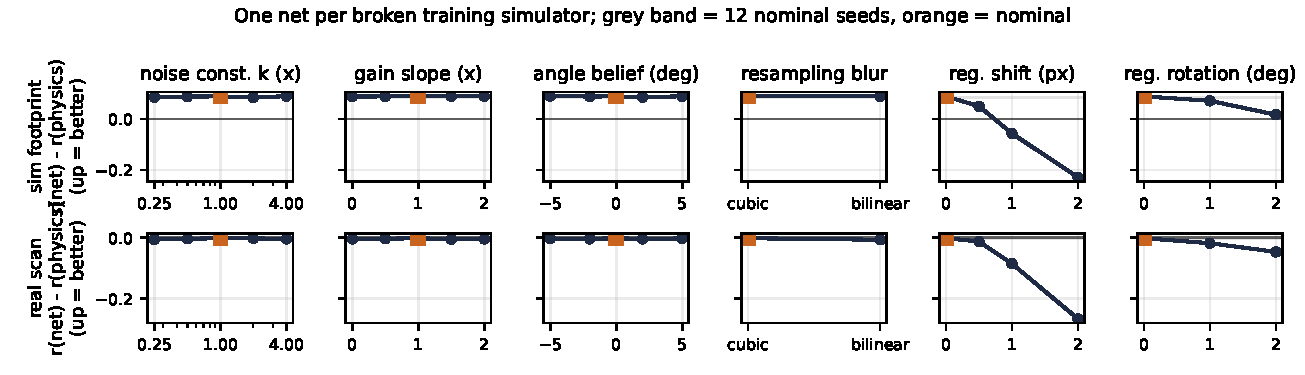
\includegraphics[width=0.72\linewidth]{wp2_tolerance_curves.pdf}
  \caption{Defect tolerance: $r(\mathrm{net})-r(\mathrm{physics})$, one network per broken training simulator, on nominal simulated cases (top: footprint, middle: hole) and the real scan (bottom). Grey band: 12 nominal seeds; orange: nominal. Geometry is the cliff; the blur defect is visible only on the real scan.}
  \label{fig:tolerance}
\end{figure}

\textbf{Tolerance ladder.} One network per deliberately broken simulator, 18 rungs across six families, all with one shared seed so that rung differences are the simulator; the 12 control members provide the seed band ($\Delta r \in [+0.082, +0.090]$ on the simulated footprint, $[-0.005, -0.002]$ on the real scan). The result (Fig.~\ref{fig:tolerance}) is asymmetric: the noise constant can be wrong by $4\times$ either way, the gain slope doubled or removed, the angle belief off by 5$^\circ$, all without leaving the band. Geometry is different: a 0.5\,px registration shift, five times the calibration uncertainty but half a pixel, already leaves the band (four seeds: $-0.013$ to $-0.005$ on the real scan); at 1\,px the network is worse than the physics inverse it refines ($-0.057$ simulated, $-0.086$ real), at 2\,px it destroys the restoration ($-0.27$ real); a 2$^\circ$ rotation costs $-0.047$. The blur rung replays Section~\ref{sec:setup} as one point on a curve: invisible on simulated tests, on the real scan it leaves the band for all four seeds, with the table's only contrast overshoot (1.013).

\textbf{Blind diagnostics.} Can the broken component be identified from one scan, without truth? We compare measurement to simulation with nine per-line statistics (level, contrast, mid- and high-band power ratios, a single-map noise-constant estimate, signed sub-pixel offsets, a differential rotation estimate, a gain-template projection). The null is the crucial choice: with noise-only pairs everything fires on the real scan (a 0.3$^\circ$ registration residual gives $z\approx60$), so we build it from pairs drawn \emph{within the calibration uncertainty}: a flag means the discrepancy exceeds what the simulator itself claims to know. With a rule fixed before the experiment, the battery identifies blur 10/10, shifts down to 0.5\,px 30/30, rotations of 1--2$^\circ$ 20/20 and noise scalings $\times$0.25/2/4 30/30, with 4/48 false alarms; gain-family defects within the calibration uncertainty are invisible by construction (0/80 pre-registered; a post-hoc template recovers only extremes; gain vs angle is degenerate at one tilt). Crossing audit and ladder gives the payoff matrix: \emph{every rung with material damage is visible, and every invisible rung is harmless} (one formal exception at 0.0002, the band's own resolution). On the real scan the battery, blind, flags our v1 simulator and the validated bilinear emulator as ``blur'' (high-frequency power ratio 1.7--2.1) and leaves the v2 simulator with one finding: a residual noise excess ($k$ ratio 1.19), i.e.\ it rediscovers the blur lesson and names the next problem (Appendix Fig.~\ref{fig:confusion}).

\section{Closing the loop: a posterior over the simulator from one scan}
\label{sec:wp4}

\begin{figure}[t]
  \centering
  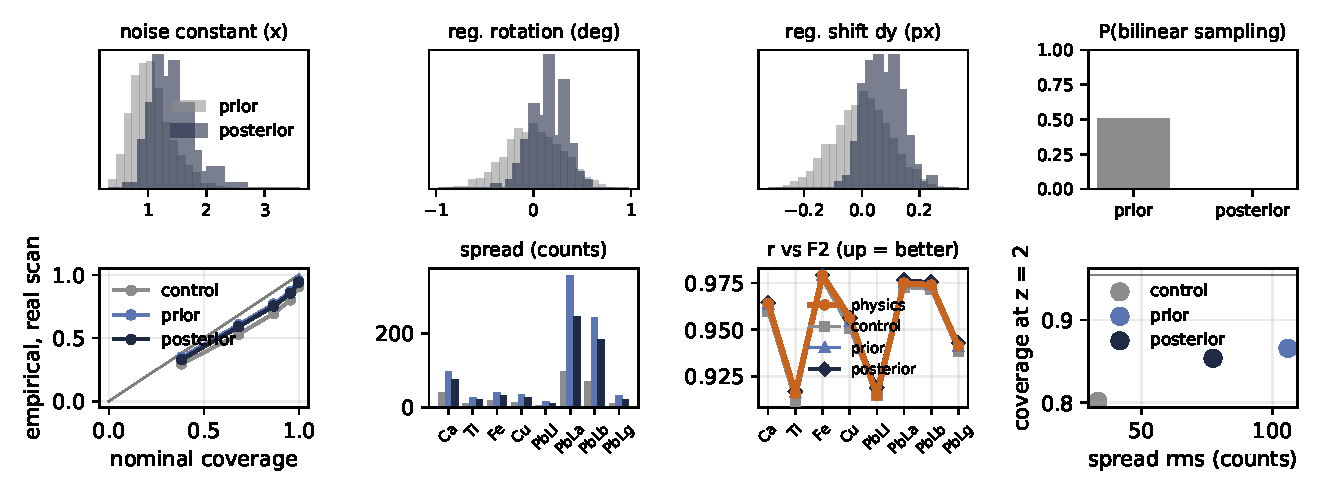
\includegraphics[width=0.72\linewidth]{wp4_prior_posterior.pdf}
  \caption{Top: prior (light) and posterior (navy) knob marginals from rejection ABC on one real scan; the v1 bilinear sampling drops from 0.5 to 0.000. Bottom: real-scan calibration, per-line spread and $r$, and the coverage-vs-width tradeoff of the three ensembles.}
  \label{fig:posterior}
\end{figure}

The audit statistics support likelihood-free inference \citep{cranmer2020}: rejection ABC \citep{beaumont2002} over the simulator's knobs, prior = the calibration jitter of Section~\ref{sec:wp1} plus the v1 bilinear sampling at probability 0.5 (the loop must reject our own mistake); 3000 draws, whitened RMS-$z$ distance, closest 5\,\% accepted (2/10\,\% agree on every direction).

\textbf{Posterior.} The bilinear defect is rejected completely (posterior 0.000); the posterior concentrates on a noisier instrument (noise scale $1.43\pm0.35$) with a small registration residual ($+0.15^\circ\pm0.17$, $+0.08\pm0.06$\,px), gains at calibration. The posterior predictive check stays honest: no draw is fully consistent (0/12), the verdict is uniformly ``noise'', and its decomposition shows a \emph{per-line} residual (real-to-simulated variance ratios 0.9--4.6 across lines) that a global noise knob cannot express. Adding the named knob (per-line noise scales, round 2) moves the marginals in the measured direction but barely deepens the fit (best whitened distance 2.02 vs a null floor of $0.95\pm0.24$) and the check still rejects: the loop converges not to perfect but to a precise statement of what is missing (unmodelled flat-field, scatter, dwell drift).

\textbf{Posterior ensemble.} Twelve networks retrained on accepted draws form the most accurate restoration in the study on the real scan: $r=0.9539$ against 0.9527 (prior), 0.9526 (physics), 0.9496 (control), at or above the physics inverse on 7/8 lines, with the smallest bias (1.07\,\%) and a 27\,\% narrower band than the prior ensemble (spread 77 vs 106 counts) at coverage 0.85/0.94 at $z=2/3$ (prior 0.87/0.95). By per-pixel Gaussian NLL, a proper score \citep{gneiting2007}, the wider prior band remains marginally better (6.45 vs 6.58 nats; control 7.27), the gap sitting exactly on the lines whose noise the knob family cannot express: one measurement bought accuracy, bias and band width, and the score prices the misspecification that remains.

\section{When does learning pay? A regime map with classical controls}
\label{sec:wp3}

\begin{figure}[t]
  \centering
  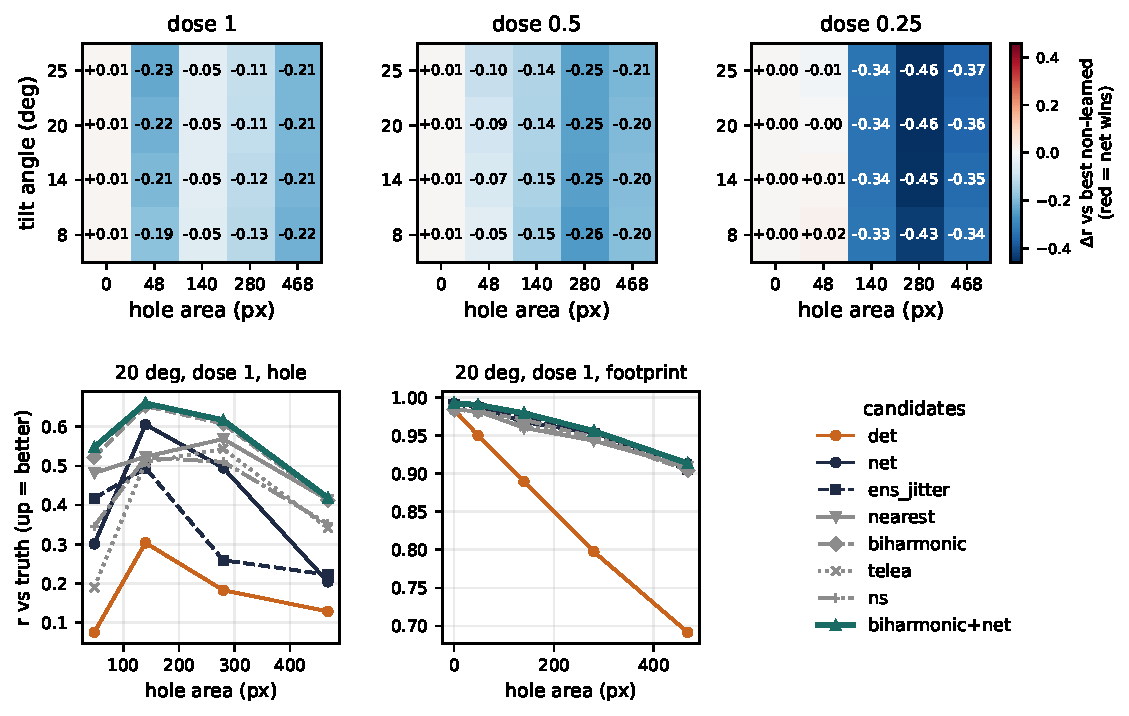
\includegraphics[width=0.7\linewidth]{wp3_regime_map.pdf}
  \caption{Left: $r(\mathrm{net})$ minus the best non-learned candidate (physics or best classical fill) inside the hole, per dose; blue = the non-learned candidate wins. Right: $r$ against hole area at 20$^\circ$, dose 1, all candidates, inside the hole and on the footprint.}
  \label{fig:regime}
\end{figure}

We sweep 180 cases (4 angles $\times$ 5 holes $\times$ 3 doses $\times$ 3 seeds, all from \Ftwo{}) and compare physics, the nominal network, the jitter-ensemble mean, and four classical fills applied in the tilted frame (nearest, biharmonic \citep{scikit-image}, Telea \citep{telea2004}, Navier--Stokes \citep{bertalmio2001}) through the same physics inverse. On measured pixels the learned candidates beat every alternative in every cell (no hole: 0.985 vs 0.977 physics; $14\times20$ hole footprint: 0.952 ensemble vs 0.937 best classical vs 0.781 physics), with a margin that grows with hole size (they also repair the warp blur around the hole). Inside the hole the ranking inverts: the biharmonic fill beats the network in 16/16 cells (0.467 vs 0.415 at 20$^\circ$/$14\times20$), and at quarter dose the learned fills collapse (0.03 and $-0.01$) while the classical fill is dose-proof (0.455). The only learned candidate that wins every hole cell is the hybrid, classical fill then network, by 0.005--0.03: the network adds sharpening, not a better fill. Hole columns are angle-independent (the measured warp does not scale with angle); what matters is hole size and dose. On this instrument the learned prior buys contrast, noise, neighbourhood repair and calibrated uncertainty, not missing content (Fig.~\ref{fig:regime}).

\section{Limitations and outlook}
\label{sec:limits}

All of this is one painting, one instrument, one real tilted scan; we claim the auditable chain, not universal numbers. The calibration sigmas are lower bounds (the one-sided gain-slope uncertainty is symmetrised), and the jitter is only as honest as they are. Ensembles have 12 members; rungs use one seed, the two borderline rungs four. Rejection ABC with $9\times8$ summaries and 22 round-2 parameters is at its resolution edge; SMC is the upgrade. The hole failure suggests training on classically filled holes; uncertainty-guided acquisition (pilot in Appendix Fig.~\ref{fig:adaptive}) is the route to less irradiation of heritage objects, our main foreseen societal benefit. Code and result tables will be released.

\begin{thebibliography}{13}

\bibitem[Alfeld et al.(2013)]{alfeld2013}
M.~Alfeld, J.~V. Pedroso, M.~van Eikema Hommes, G.~Van~der Snickt, G.~Tauber, J.~Blaas, M.~Haschke, K.~Erler, J.~Dik, and K.~Janssens.
\newblock A mobile instrument for in situ scanning macro-XRF investigation of historical paintings.
\newblock \emph{Journal of Analytical Atomic Spectrometry}, 28(5):760--767, 2013.

\bibitem[Beaumont et al.(2002)]{beaumont2002}
M.~A. Beaumont, W.~Zhang, and D.~J. Balding.
\newblock Approximate Bayesian computation in population genetics.
\newblock \emph{Genetics}, 162(4):2025--2035, 2002.

\bibitem[Bertalmio et al.(2001)]{bertalmio2001}
M.~Bertalmio, A.~L. Bertozzi, and G.~Sapiro.
\newblock Navier--Stokes, fluid dynamics, and image and video inpainting.
\newblock In \emph{IEEE CVPR}, 2001.

\bibitem[Cranmer et al.(2020)]{cranmer2020}
K.~Cranmer, J.~Brehmer, and G.~Louppe.
\newblock The frontier of simulation-based inference.
\newblock \emph{PNAS}, 117(48):30055--30062, 2020.

\bibitem[Gneiting and Raftery(2007)]{gneiting2007}
T.~Gneiting and A.~E. Raftery.
\newblock Strictly proper scoring rules, prediction, and estimation.
\newblock \emph{Journal of the American Statistical Association}, 102(477):359--378, 2007.

\bibitem[Ilg et al.(2018)]{ilg2018}
E.~Ilg, {\"O}.~{\c{C}}i{\c{c}}ek, S.~Galesso, A.~Klein, O.~Makansi, F.~Hutter, and T.~Brox.
\newblock Uncertainty estimates and multi-hypotheses networks for optical flow.
\newblock In \emph{ECCV}, 2018.

\bibitem[Kingma and Ba(2015)]{kingma2015}
D.~P. Kingma and J.~Ba.
\newblock Adam: A method for stochastic optimization.
\newblock In \emph{ICLR}, 2015.

\bibitem[Lakshminarayanan et al.(2017)]{lakshminarayanan2017}
B.~Lakshminarayanan, A.~Pritzel, and C.~Blundell.
\newblock Simple and scalable predictive uncertainty estimation using deep ensembles.
\newblock In \emph{NeurIPS}, 2017.

\bibitem[Ronneberger et al.(2015)]{ronneberger2015}
O.~Ronneberger, P.~Fischer, and T.~Brox.
\newblock U-Net: Convolutional networks for biomedical image segmentation.
\newblock In \emph{MICCAI}, 2015.

\bibitem[Telea(2004)]{telea2004}
A.~Telea.
\newblock An image inpainting technique based on the fast marching method.
\newblock \emph{Journal of Graphics Tools}, 9(1):23--34, 2004.

\bibitem[Tobin et al.(2017)]{tobin2017}
J.~Tobin, R.~Fong, A.~Ray, J.~Schneider, W.~Zaremba, and P.~Abbeel.
\newblock Domain randomization for transferring deep neural networks from simulation to the real world.
\newblock In \emph{IEEE/RSJ IROS}, 2017.

\bibitem[van der Walt et al.(2014)]{scikit-image}
S.~van~der Walt, J.~L. Sch{\"o}nberger, J.~Nunez-Iglesias, F.~Boulogne, J.~D. Warner, N.~Yager, E.~Gouillart, and T.~Yu.
\newblock scikit-image: image processing in Python.
\newblock \emph{PeerJ}, 2:e453, 2014.

\end{thebibliography}

\appendix

\section{Training and evaluation details}
\label{app:training}

\paragraph{Data and protocol.} Frontal maps are $60\times120$, the tilted frame $45\times80$; the tilted footprint covers 3466 of the 7200 frontal pixels. Training pairs are simulated from \Fone{} only: random tilt angle in $[4^\circ, 25^\circ]$, random flips, 25\,\% low-dose samples ($\times$0.35--1.0), 30\,\% of samples with 1--2 zeroed dropout blocks of 8--17\,px in the tilted frame, recorded in a validity channel. The network input is the deterministic physics inverse of the simulated tilted scan (8 element channels, per-line normalisation fixed from \Fone{}), plus validity and angle channels; the target is the frontal map. Four fixed $15\times30$ spatial blocks of the frontal frame are excluded from the training loss and serve early stopping. \Ftwo{} and the real scan \Treal{} are never used in training; all final numbers are computed against \Ftwo{} as reference, on the footprint and, where applicable, inside the dropout hole. Metrics: Pearson $r$, SSIM, level bias in percent, and the contrast ratio $\mathrm{CV(candidate)}/\mathrm{CV(reference)}$.

\paragraph{Architecture and optimisation.} Residual U-Net, three resolution levels, base width 32, GroupNorm and SiLU, 469k parameters, $1\times1$ zero-initialised head (the untrained model equals the physics inverse). Adam \citep{kingma2015} with learning rate $10^{-3}$, batch 8, at most 1500 steps, validation every 50 steps on a fixed simulated set (8 angles $\times$ 3 replicates), early stopping after 10 validations without improvement, plateau learning-rate decay. One training run takes about 10 minutes on a 12-core CPU workstation; no GPUs were used anywhere. The study trains 60 networks in total (12 jitter, 12 control, 18 ladder rungs, 6 extra-seed variants, 12 posterior members), about 10 CPU-hours, plus inference-only sweeps.

\paragraph{Seeds and error bars.} The two ensembles share their twelve seeds, so jitter-vs-control differences are attributable to the simulator draw; every ladder rung uses the seed of one control member, and the 12 control members define the initialisation band shown in Fig.~\ref{fig:tolerance}; the two borderline rungs (0.5\,px shift, blur) were re-trained with three extra seeds each and their real-scan damage holds for every seed. Coverage error bars are standard deviations over lines and cases. The aleatoric band term uses 8 noise re-simulations per case; the reference-noise term uses the calibrated $k_{\mathrm{el}}$.

\section{Additional figures}
\label{app:figures}

\begin{figure}[h]
  \centering
  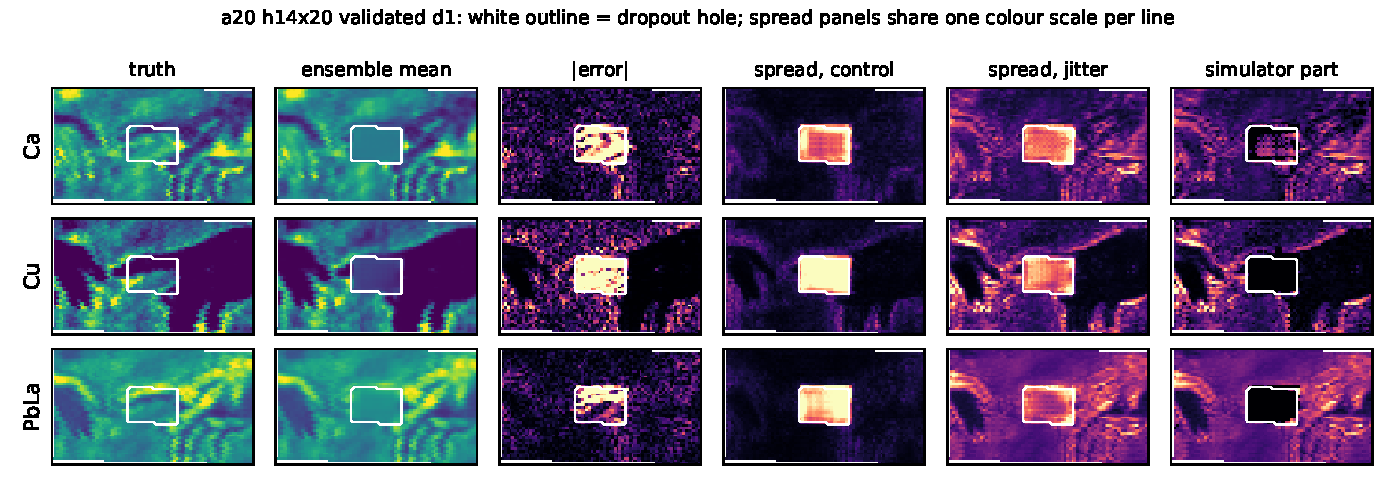
\includegraphics[width=\linewidth]{wp1_spread_maps.pdf}
  \caption{Spread maps on the harsh case (20$^\circ$, $14\times20$ hole, white outline), three lines. Columns: reference, jitter-ensemble mean, absolute error, control spread, jitter spread, and the simulator part $\sqrt{\max(\sigma_{\mathrm{jitter}}^2-\sigma_{\mathrm{control}}^2,0)}$; the three spread panels of a line share one colour scale. The control spread lives in the hole; the jitter spread follows the painting's structure; inside the hole the jitter ensemble is narrower than the control (dark).}
  \label{fig:spreadmaps}
\end{figure}

\begin{figure}[h]
  \centering
  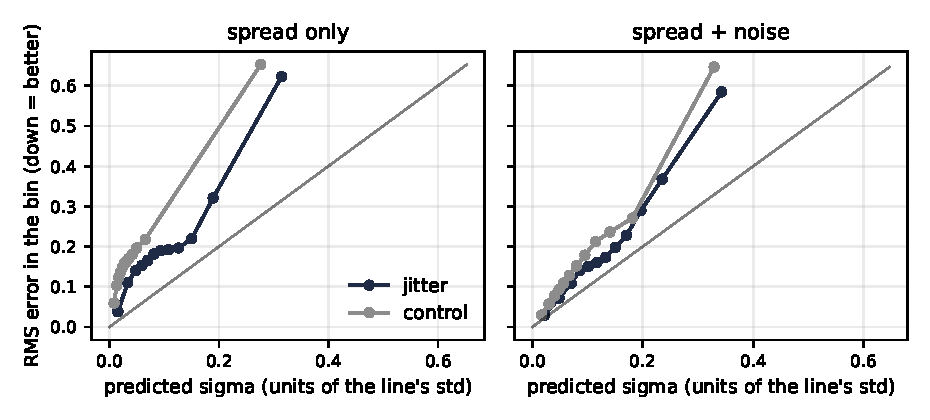
\includegraphics[width=0.8\linewidth]{wp1_error_vs_sigma.pdf}
  \caption{Binned reliability: RMS error against predicted $\sigma$ in twelve $\sigma$-quantile bins, pooled over simulated cases and lines in units of each line's standard deviation; diagonal = calibrated. Left: ensemble spread only; right: spread plus propagated noise.}
  \label{fig:reliability}
\end{figure}

\begin{figure}[h]
  \centering
  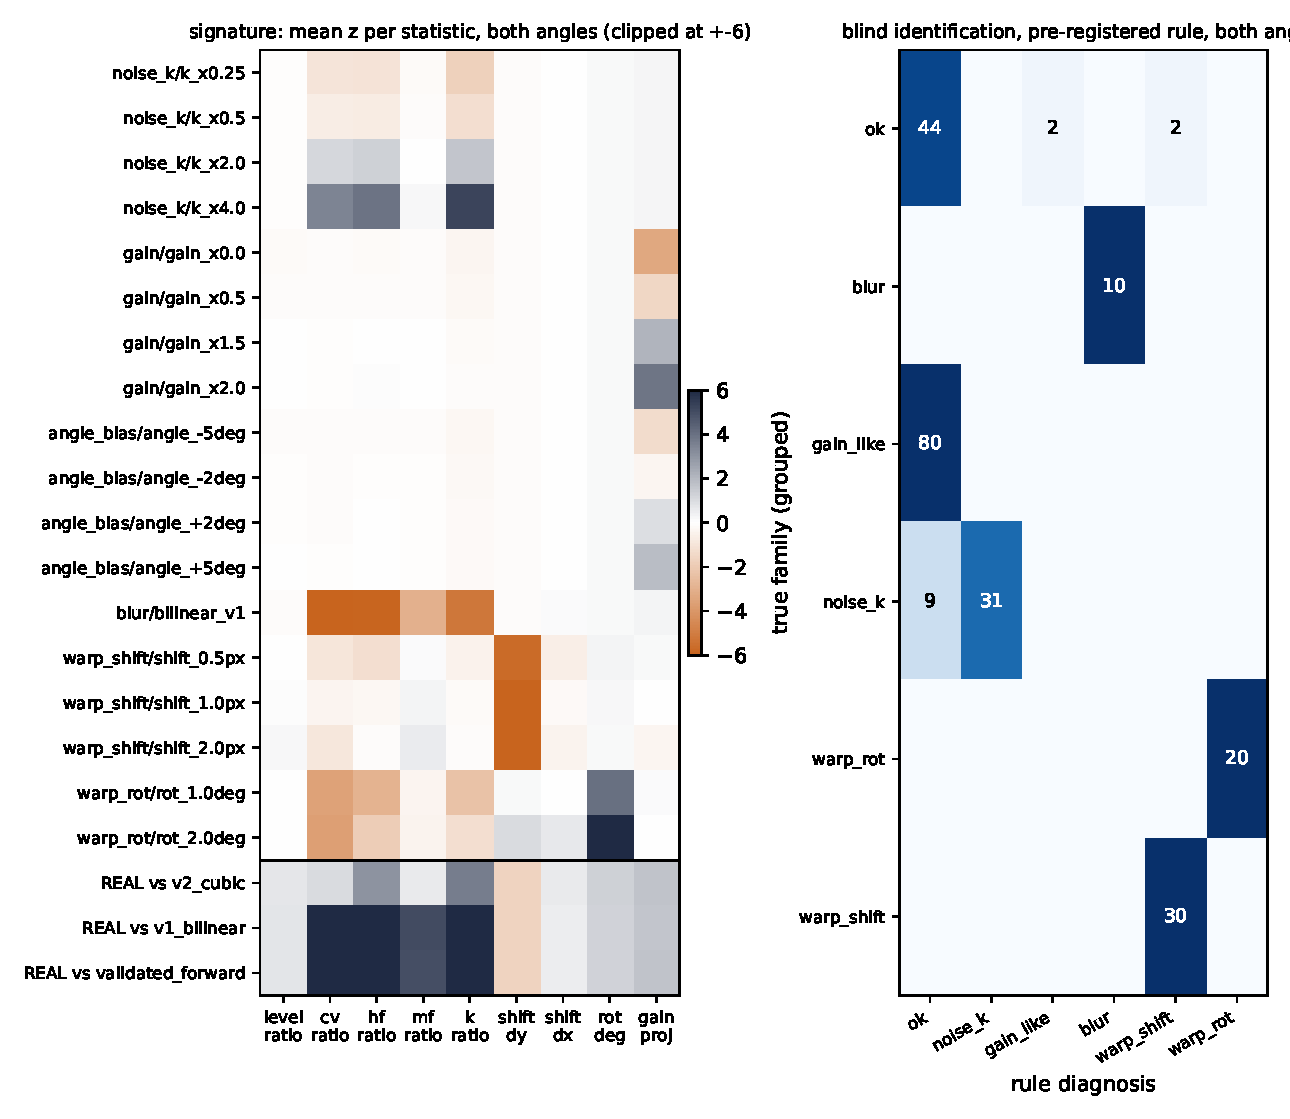
\includegraphics[width=\linewidth]{wp2_diag_confusion.pdf}
  \caption{Blind diagnostics. Left: signature of every defect rung, the mean $z$ of each statistic against the calibration-uncertainty null (both test angles pooled, clipped at $\pm6$); the bottom block is the real scan against three simulators (v2 cubic, v1 bilinear, validated bilinear emulator). Right: identification counts of the pre-registered rule, true family (grouped) versus diagnosis.}
  \label{fig:confusion}
\end{figure}

\begin{figure}[h]
  \centering
  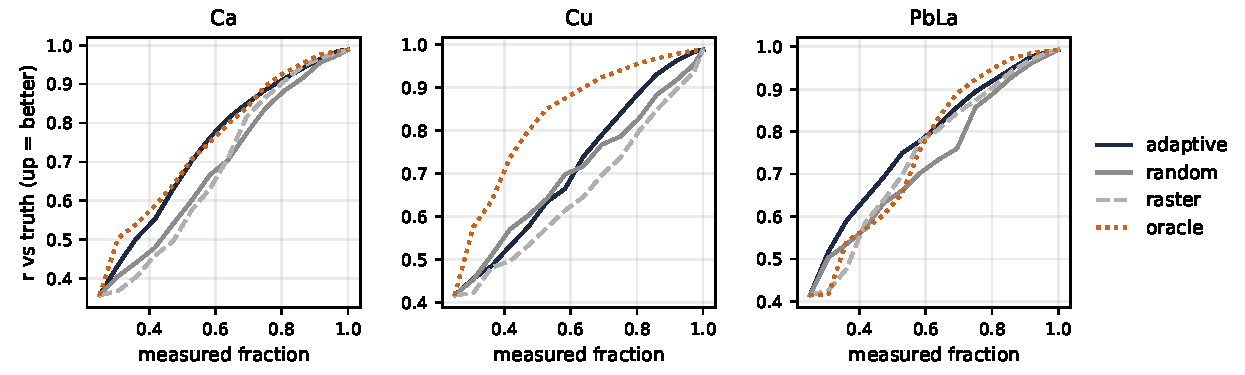
\includegraphics[width=\linewidth]{wp1_adaptive.pdf}
  \caption{Uncertainty-guided acquisition pilot: $r$ against the measured fraction of the tilted frame when $5\times5$ tiles are acquired in the order of the jitter-ensemble spread (adaptive), at random, in raster order, or by the true error (oracle, not realisable); 8 tiles per step from a 25\,\% start, mean of three simulated cases. Adaptive reaches $r\ge0.90$ (mean over Ca, Cu, Pb\,L$\alpha$) after measuring 79\,\% of the frame, against 85\,\% for random or raster order and 72\,\% for the oracle; for $r\ge0.95$ the fractions are 88\,\%, 93\,\% and 82\,\%.}
  \label{fig:adaptive}
\end{figure}

\clearpage
\input{checklist}

\end{document}
